\documentclass{article}
%przykladowe pakiety
\usepackage[utf8]{inputenc}
\usepackage{polski}
\usepackage{graphicx}
\usepackage{amsmath} % w zasadzie tez mozna wywalic 
\usepackage{booktabs}
\usepackage{listings}
\usepackage{color}


% przykladowe kolorowanie kodu w listingu
\lstset{language=C++,backgroundcolor=\color[rgb]{0.99,0.99,0.99},captionpos=b,tabsize=3,numbers=left,numberstyle=\tiny,numbersep=5pt,basicstyle=\footnotesize,keywordstyle=\color[rgb]{0,0,1},commentstyle=\color{Darkgreen},stringstyle=\color{red},numbers=left,xleftmargin=2em,framexleftmargin=1.8em,}



\begin{document}

%strona tytulowa - osobny plik
\begin{titlepage}
    \newcommand{\HRule}{\rule{\linewidth}{0.5mm}}
    \center
    
\includegraphics[scale=0.4]{logo.jpg}\\[1cm] 
    \HRule \\[0.8cm]
    { \Large \bfseries 	 Projektowanie efektywnych algorytmów }\\[0.4cm]
    \HRule \\[1.5cm]
    { \Large \bfseries Projekt \textit{1}}\\[0.4cm]
    \textbf{ }
    \vspace{10mm} 
    
    \begin{minipage}{0.4\textwidth}
    \begin{flushleft} \large
    \end{flushleft}
    \end{minipage}
    \begin{minipage}{0.5\textwidth}
    \begin{flushright} \large
    \vfill
    \vspace{10mm} % mm vertical space
    \par Wydział Elektroniki
    \par Kierunek: Informatyka
    \vfill
    \par Paweł \textsc{Szynal 226026} \\
    \vspace{10mm} % mm vertical space
   \vspace{10mm} % mm vertical space
   \par Prowadzący:\\ mgr inż. Antoni Sterna
    \end{flushright}
    \end{minipage}\\[3cm]
     {\large Wrocław 2020 r.}\\[2cm]
\end{titlepage}
   
\newpage
    
\tableofcontents
\newpage

\section{Wstęp}

Celem projektu było wykonanie programu, wykorzystującego algorytmy programowania dynamicznego, podziału i ograniczeń oraz przeglądu zupełnego do rozwiązania problemu komiwojażera
(ang. Travelling Salesman Problem).

\section{Specyfikacja techniczna}

\begin{itemize}
\item Program został wykonany obiektowo w języku c++
\item Program akceptuje dane w postaci macierzy odległości
\item Czas wykonania algorytmów mierzone był przy wykorzystaniu bibliotek systemowych
\item do dynamicznego przechowywania danych została wykorzystana biblioteka $Vector$

\end{itemize}

\section{Analiza problemu}

Problem komiwojażera należy do klasy problemów NP-trudnych. Jest to
optymalizacyjny problem, rozwiązaniem którego jest znalezienie minimalnego cyklu Hamiltona
(ścieżki prowadzącej przez wszystkie wierzchołki grafu, powracając na końcu do wierzchołka
początkowego). W wersji asynchronicznej, odległości pomiędzy
wierzchołkami mogą dodatkowo zależeć także od kierunku przejścia pomiędzy nimi. Główną
trudnością w rozwiązaniu problemu jest znacząca liczba możliwych kombinacji.


\section{Opis Algorytmów}

\subsection{Przegląd zupełny}

Algorytm przeglądu zupełnego (ang. brute force) polega na przeanalizowaniu wszystkich
możliwych przypadków, oraz wybraniu tego o najlepszej wartości. Zaletą tego algorytmu jest pewność,
że otrzymany wynik jest najlepszym rozwiązaniem problemu. Poważną jego wadą jest jednak
złożoność czasową wynoszącą $O(n!)$, co w praktyce czyni ten algorytm bezużytecznym dla większych
zbiorów danych. Zaimplementowany został algorytm przeszukiwania w głąb wywoływany rekurencyjnie ze zmiennymi śledzącymi najkrótszą drogę i koszt.\\\\\\

\subsection{Metoda podziału i ograniczeń}

Metoda polega przechodzeniu w głąb problemu przy jednoczesnym obliczaniu minimum - $upperBound$ (poprzez metodę redukcji macierzy). Po znalezieniu pierwszej drogi zostaje zaktualizowana wartość $lowerBound$ i wyeliminowane wszystkie elementy które posiadają wartość $upperBound$ większą od $lowerBound$. Minusem tego algorytmu jest duża złożoność pamięciowa, gdyż dla każdego elementu tworzymy uaktualnioną dla danego elementu kopię macierzy kosztów przejścia pomiędzy wierzchołkami. W najgorszym przypadku odwiedzimy każdy wierzchołek, tak jak przy przeglądzie zupełnym.\\\\\\\\\\\\\\\\\\



\section{Pomiary i wnioski}
Każdy pomiar został wykonany dziesięciokrotni, a potem uśredniony.

    	\begin{figure}[h]
			\begin{center}
      			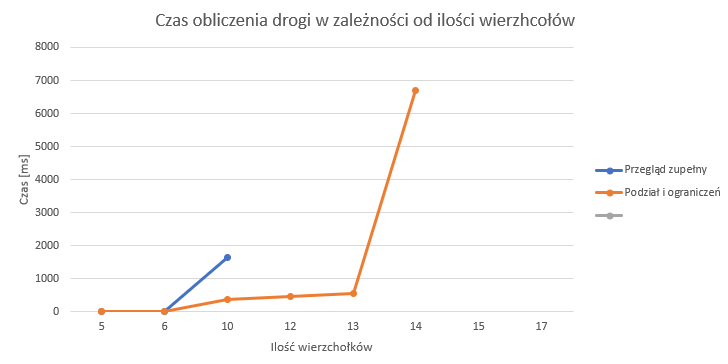
\includegraphics[width=1\textwidth]{./w.jpg}
      				\caption{Pomiary w [ms] w zależności od ilości wierzchołków}
      			\label{fig:obraz}
			\end{center}
		\end{figure}

Jak widać algorytmy przeglądu zupełnego i podziału i ograniczeń okazują się nieefektywne już przy odpowiednio 12 i 15 wierzchołkach. Ponadto algorytm podziałów i ograniczeń mimo większej wydajności zużywa dużo więcej pamięci, a jego szybkość nie jest stała - zależna od grafu jak i ilości wierzchołków grafu. 

\end{document}

